\section{Présentation}

%%%%%%%%%%%%%%%%%%%%%%%%%%%%%%%%%%%%%%%%%%%%%%%%%%%%%%%%%%%%%%%%%%%%%%%%%%%%%%%%

\begin{frame}[fragile]{Histoire brève de PostgreSQL - POSTGRES}

   \begin{itemize}
      \item PostgreSQL est dérivé du projet POSTGRES amorcé par l'Université de Californie à Berkeley
      \item POSTGRES est né en 1986 et a été financé par:
      \begin{itemize}
         \item le DARPA (Defense Advanced Research Projects Agency)
         \item l'ARO (Army Research Office)
         \item le NSF (National Science Foundation)
         \item ESL Inc.
      \end{itemize}
      \item POSTGRES a été utilisé par différents projets universitaires.
      \item Illustra Information Technologies qui a fusionné avec Informix, rachetée par IBM commercialise le code dans les années 90
   \end{itemize}

\begin{toile}
\toileurl{https://www.postgresql.org/docs/15/history.html}
\end{toile}

\end{frame}

%%%%%%%%%%%%%%%%%%%%%%%%%%%%%%%%%%%%%%%%%%%%%%%%%%%%%%%%%%%%%%%%%%%%%%%%%%%%%%%%

\begin{frame}[fragile]{Postgres95}

   \begin{itemize}
      \item En 1993, la communauté d'utilisateurs double de taille.
      \item La maintenance du projet devient très chronophage pour les équipes de recherche universitaires qui décident de mettre fin au projet avec la publication finale de la version 4.2
      \item En 1994, Andrew Yu et Jolly Chen ajoutent un interpréteur SQL à POSTGRES
      \item Le projet change de nom pour devenir Postgres95, l'héritier open source de POSTGRES
      \item Postgres95 est entièrement écrit en ANSI C et son code est réduit de 25\%.
      \item Postgres95 v1.0 est 30-50\% plus rapide que POSTGRES
   \end{itemize}

\end{frame}

%%%%%%%%%%%%%%%%%%%%%%%%%%%%%%%%%%%%%%%%%%%%%%%%%%%%%%%%%%%%%%%%%%%%%%%%%%%%%%%%

\begin{frame}[fragile]{PostgreSQL}

   \begin{itemize}
      \item Le langage PostQUEL est définitivement abandonné au profit de SQL
      \item Le client psql est développé. Il utilise la librairie GNU readline
      \item Le support des grands objets (Large Objects) est mis en place
      \item En 1996, Postgres95 devient PostgreSQL car il semble important que l'année ne figure pas dans le nom
      \item Il est aussi possible de l'appeler Postgres (en référence à son ancêtre)
   \end{itemize}

\end{frame}

%%%%%%%%%%%%%%%%%%%%%%%%%%%%%%%%%%%%%%%%%%%%%%%%%%%%%%%%%%%%%%%%%%%%%%%%%%%%%%%%

\begin{frame}[fragile]{Exercice - Installer PostgreSQL 15 sur les serveurs de formation}

   \begin{itemize}
      \item Installer le serveur PostgreSQL sur les serveurs \textbf{hqpg-0x} et \textbf{hqpg-0x-repl}
      \item Les serveurs ont pour OS Rocky Linux version 8
   \end{itemize}

\begin{toile}
\toileurl{https://www.postgresql.org/download/linux/redhat/}
\toileurl{https://rockylinux.org/}
\end{toile}

\end{frame}

%%%%%%%%%%%%%%%%%%%%%%%%%%%%%%%%%%%%%%%%%%%%%%%%%%%%%%%%%%%%%%%%%%%%%%%%%%%%%%%%

\section{Ecosystème}

\begin{frame}{Présentation de l'écosystème PostgreSQL}

   \begin{itemize}
      \item La communauté PostgreSQL met à disposition un nombre assez important d'outils pour faciliter la vie des utilisateurs et des administrateurs
      \item Les outils suivants vont être présentées durant cette formation:
      \begin{itemize}
         \item POWA
         \item pgBadger
         \item pgAdmin4
      \end{itemize}
   \end{itemize}


\end{frame}

%%%%%%%%%%%%%%%%%%%%%%%%%%%%%%%%%%%%%%%%%%%%%%%%%%%%%%%%%%%%%%%%%%%%%%%%%%%%%%%%

\begin{frame}{POWA}

   \begin{itemize}
      \item PoWA signifie "PostgreSQL Workload Analyzer"
      \item Il supporte PostgreSQL 9.4+
      \item PoWA permet de collecter, agréger et purger des statistiques sur plusieurs instances PostgreSQL depuis plusieurs extensions statistiques
      \item En fonction des besoins de l'utilisateur, PoWA fonctionne avec 2 modes:
   \begin{itemize}
         \item en utilisant le \textbf{background worker}. Ce fonctionnement est adapté aux environnements mono instances. Il nécessite un redémarrage de la base.
         \item en utilisant le \textbf{PoWA collector}. Ne nécessite pas de redémarrage, collecte les informations depuis plusieurs bases, le standby inclus
   \end{itemize}

   \end{itemize}

\begin{tiny}
\begin{toile}
\toileurl{https://powa.readthedocs.io/en/latest/}
\end{toile}
\end{tiny}

\end{frame}

%%%%%%%%%%%%%%%%%%%%%%%%%%%%%%%%%%%%%%%%%%%%%%%%%%%%%%%%%%%%%%%%%%%%%%%%%%%%%%%%

\begin{frame}{POWA - modules de statistiques}

   \begin{itemize}
      \item Les modules de statistiques supportés par PoWA sont:
      \begin{itemize}
         \item \textbf{pg\_stat\_statements} fournit des informations sur les requêtes en cours d'exécution
         \item \textbf{pg\_qualstats} fournit des informations sur les prédicats ou les clauses \textbf{where}
         \item \textbf{pg\_stat\_kcache} fournit des informations sur le cache de l'OS
         \item \textbf{pg\_wait\_sampling} fournit des informations sur les événements en attente
         \item \textbf{pg\_track\_settings} suit et garde une trace des modifications du paramétrage du serveur PostgreSQL
      \end{itemize}
      \item Il est également possible d'ajouter le support de HypoPG
      \item HypoPG permet de tester des index sans avoir à les déployer réellement en base
   \end{itemize}

\end{frame}

%%%%%%%%%%%%%%%%%%%%%%%%%%%%%%%%%%%%%%%%%%%%%%%%%%%%%%%%%%%%%%%%%%%%%%%%%%%%%%%%

\begin{frame}{POWA - les composants logiciels}

   \begin{itemize}
      \item \textbf{PoWA-archivist}: extension PostgreSQL de collecte des statistiques
      \item \textbf{PoWA-collector}: démon de collecte des informations des instances distantes de PostgreSQL
      \item \textbf{PoWA-web}: interface web de PoWA
   \end{itemize}

   Remarque: Il est préférable de ne pas déployer PoWA sur un environnement de production car les performances peuvent être négativement impactés

\end{frame}

%%%%%%%%%%%%%%%%%%%%%%%%%%%%%%%%%%%%%%%%%%%%%%%%%%%%%%%%%%%%%%%%%%%%%%%%%%%%%%%%

\begin{frame}[fragile]{POWA - Exercice }

   \begin{itemize}
      \item Déployer PoWA en suivant le lien: https://powa.readthedocs.io/en/latest/quickstart.html
   \end{itemize}

\begin{tiny}
\begin{Verbatim}[commandchars=\\\{\}]
[root@localhost ~]# dnf install postgresql15-contrib
[root@localhost ~]# dnf install powa_15 pg_qualstats_15 pg_stat_kcache_15 hypopg_15
\end{Verbatim}
\end{tiny}

   Modifier la ligne suivante dans \textbf{postgresql.conf}:

\begin{tiny}
\begin{Verbatim}[commandchars=\\\{\}]
shared_preload_libraries = 'pg_stat_statements,powa,pg_stat_kcache,pg_qualstats,hypopg'
\end{Verbatim}
\end{tiny}

Puis redémarrer le service PostgreSQL:
\begin{tiny}
\begin{Verbatim}[commandchars=\\\{\}]
[root@localhost ~]# systemctl restart postgresql-15.service
\end{Verbatim}
\end{tiny}

\end{frame}

%%%%%%%%%%%%%%%%%%%%%%%%%%%%%%%%%%%%%%%%%%%%%%%%%%%%%%%%%%%%%%%%%%%%%%%%%%%%%%%%

\begin{frame}[fragile]{POWA - Exercice - Installation des extensions}

\begin{tiny}
\begin{Verbatim}[commandchars=\&\{\}]
[root@localhost ~]# su - postgres
Dernière connexion : mercredi 22 février 2023 à 13:16:44 EST sur pts/1
[postgres@localhost ~]$ psql
psql (15.2)
Saisissez « help » pour l'aide.

postgres=# CREATE DATABASE powa;
CREATE DATABASE
postgres=# \c powa
Vous êtes maintenant connecté à la base de données « powa » en tant qu'utilisateur « postgres ».
powa=# CREATE EXTENSION pg_stat_statements;
CREATE EXTENSION
powa=# CREATE EXTENSION btree_gist;
CREATE EXTENSION
powa=# CREATE EXTENSION powa;
CREATE EXTENSION
postgres=# CREATE EXTENSION hypopg;
CREATE EXTENSION
postgres=# CREATE ROLE powa SUPERUSER LOGIN PASSWORD 'astrongpassword' ;
CREATE ROLE
\end{Verbatim}
\end{tiny}

\end{frame}

%%%%%%%%%%%%%%%%%%%%%%%%%%%%%%%%%%%%%%%%%%%%%%%%%%%%%%%%%%%%%%%%%%%%%%%%%%%%%%%%

\begin{frame}[fragile]{POWA - Exercice - Installation de l'interface web}

   Installer le paquet powa\_15-web:
\begin{tiny}
\begin{Verbatim}[commandchars=\&\{\}]
[root@localhost ~]# dnf install powa_15-web
\end{Verbatim}
\end{tiny}

   Créer le fichier \textbf{/etc/powa-web.conf}:
\begin{tiny}
\begin{Verbatim}[commandchars=\&\#\#]
servers={
  'main': {
    'host': 'localhost',
    'port': '5432',
    'database': 'powa'
  }
}
cookie_secret="linagora"
\end{Verbatim}
\end{tiny}

\begin{tiny}
\begin{Verbatim}[commandchars=\&\{\}]
[root@localhost ~]# powa-web
[I 230222 18:01:27 powa-web:13] Starting powa-web on http://0.0.0.0:8888/
\end{Verbatim}
\end{tiny}

Pour accéder au serveur web depuis le PC, merci de créer le tunnel SSH équivalent avec PuttY:
\begin{tiny}
\begin{Verbatim}[commandchars=\\\{\}]
# ssh -L 8888:10.10.10.28:8888 hqpg-sandbox
\end{Verbatim}
\end{tiny}

Puis entrer l'URL:
\begin{tiny}
\begin{Verbatim}[commandchars=\\\{\}]
http://localhost:8888/
\end{Verbatim}
\end{tiny}

\end{frame}

%%%%%%%%%%%%%%%%%%%%%%%%%%%%%%%%%%%%%%%%%%%%%%%%%%%%%%%%%%%%%%%%%%%%%%%%%%%%%%%%

\begin{frame}{POWA - Login}

   Fenêtre de login

\begin{figure}
\begin{center}
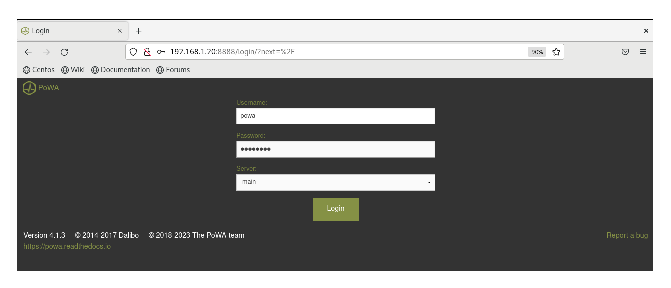
\includegraphics[angle=0, width=0.5\textwidth]{images/powa_login.eps}
\end{center}
\end{figure}

\end{frame}

%%%%%%%%%%%%%%%%%%%%%%%%%%%%%%%%%%%%%%%%%%%%%%%%%%%%%%%%%%%%%%%%%%%%%%%%%%%%%%%%

\begin{frame}{POWA - Ajout d'une base de données}

\begin{figure}
\begin{center}
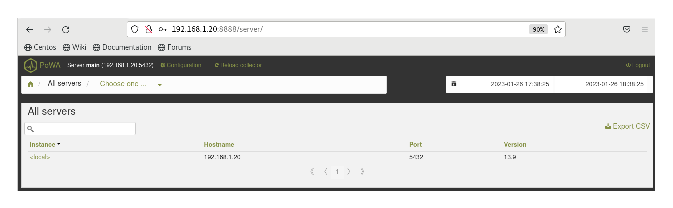
\includegraphics[angle=0, width=0.5\textwidth]{images/powa_ajout_base1.eps}
\end{center}
\end{figure}

\begin{figure}
\begin{center}

\includegraphics[angle=0, width=0.5\textwidth]{images/powa_ajout_base2.eps}
\end{center}
\end{figure}


\end{frame}

%%%%%%%%%%%%%%%%%%%%%%%%%%%%%%%%%%%%%%%%%%%%%%%%%%%%%%%%%%%%%%%%%%%%%%%%%%%%%%%%

\begin{frame}{POWA - Visualisation des métriques}

\begin{figure}
\begin{center}

\includegraphics[angle=0, width=0.5\textwidth]{images/powa_metrics1.eps}
\end{center}
\end{figure}

\begin{figure}
\begin{center}
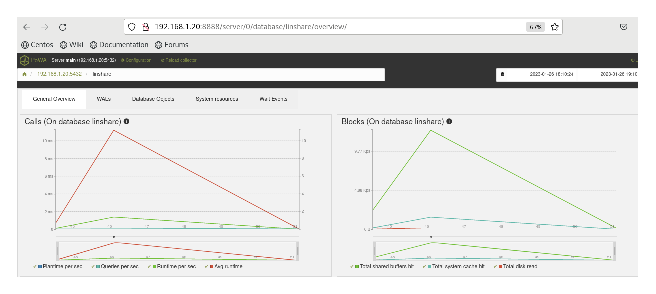
\includegraphics[angle=0, width=0.5\textwidth]{images/powa_metrics2.eps}
\end{center}
\end{figure}

\end{frame}

%%%%%%%%%%%%%%%%%%%%%%%%%%%%%%%%%%%%%%%%%%%%%%%%%%%%%%%%%%%%%%%%%%%%%%%%%%%%%%%%

\begin{frame}{pgBadger}

   \begin{itemize}
      \item pgBadger est un analyseur de logs rapide
      \item Il accepte un ou plusieurs fichiers de logs
      \item Il traite également les données fournies par l'entrée standard
      \item Il est capable de traiter un fichier de logs à distance avec un accès SSH sans mot de passe
      \item pgBadger s'appuie sur les protocoles http et ftp pour traiter les fichiers de log distants
      \item Il peut traiter les logs de pgBouncer
      \item Traitement incrémental des logs
      \item Génère des rapports au format HTML

   \end{itemize}

\begin{tiny}
\begin{toile}
\toileurl{https://pgbadger.darold.net/documentation.html}
\end{toile}
\end{tiny}

\end{frame}

%%%%%%%%%%%%%%%%%%%%%%%%%%%%%%%%%%%%%%%%%%%%%%%%%%%%%%%%%%%%%%%%%%%%%%%%%%%%%%%%

\begin{frame}{Métriques remontées par pgBadger}

   Les métriques suivantes sont remontées par pgBadger:
   \begin{itemize}
      \item Statistiques globales
      \item Requêtes les plus fréquemment en attente
      \item Requêtes ayant attendu le plus longtemps
      \item Requêtes ayant généré le plus fréquemment des fichiers temporaires
      \item Requêtes ayant généré les plus grands fichiers temporaires
      \item Requêtes les plus lentes
      \item Requêtes ayant duré le plus longtemps
      \item Requêtes les plus fréquentes
   \end{itemize}

\end{frame}

%%%%%%%%%%%%%%%%%%%%%%%%%%%%%%%%%%%%%%%%%%%%%%%%%%%%%%%%%%%%%%%%%%%%%%%%%%%%%%%%

\begin{frame}{Métriques remontées par pgBadger}

   \begin{itemize}
      \item Erreurs les plus fréquentes
      \item Histogramme du temps pris par les requêtes
      \item Histogramme du temps pris par les sessions
      \item Utilisateurs des requêtes les plus fréquentes
      \item Applications des requêtes les plus fréquentes
      \item Requêtes générant le plus d'annulation
      \item Requêtes les plus annulées
      \item Requêtes de type prepare/bind durant le plus longtemps
   \end{itemize}

\end{frame}

%%%%%%%%%%%%%%%%%%%%%%%%%%%%%%%%%%%%%%%%%%%%%%%%%%%%%%%%%%%%%%%%%%%%%%%%%%%%%%%%

\begin{frame}[fragile]{Exercice - Installer pgBadger}

   Installer pgBadger en appliquant les commandes suivantes en tant que \textbf{root}:


\begin{tiny}
\begin{Verbatim}[commandchars=\&\{\}]
[root@localhost ~]# dnf install https://dl.fedoraproject.org/pub/epel/epel-release-latest-8.noarch.rpm
[root@localhost ~]# dnf install https://dl.fedoraproject.org/pub/epel/epel-next-release-latest-8.noarch.rpm
[root@localhost ~]# dnf install perl-Text-CSV_XS
[root@localhost ~]# dnf install pgbadger
\end{Verbatim}
\end{tiny}

\end{frame}

%%%%%%%%%%%%%%%%%%%%%%%%%%%%%%%%%%%%%%%%%%%%%%%%%%%%%%%%%%%%%%%%%%%%%%%%%%%%%%%%

\begin{frame}[fragile]{Exercice - Paramétrage préalable de PostgreSQL}

   Vérifier que la ligne suivante est présente dans postgresql.conf:

\begin{tiny}
\begin{Verbatim}[commandchars=\\\{\}]
log_min_duration_statement = 0
\end{Verbatim}
\end{tiny}

Les lignes du journal doivent avoir un minimum d'information:

\begin{tiny}
\begin{Verbatim}[commandchars=\\\{\}]
log_line_prefix = '%t [%p]: '
log_checkpoints = on
log_connections = on
log_disconnections = on
log_lock_waits = on
log_temp_files = 0
log_autovacuum_min_duration = 0
log_error_verbosity = default
\end{Verbatim}
\end{tiny}

   \textbf{Remarques:}
\begin{itemize}
   \item Ne pas activer l'option log\_statement car son format ne peut être traité par pgBadger
   \item pgBadger est restreint aux messages de log en anglais. Il ne peut traiter des logs en langue française.
\end{itemize}

\end{frame}

%%%%%%%%%%%%%%%%%%%%%%%%%%%%%%%%%%%%%%%%%%%%%%%%%%%%%%%%%%%%%%%%%%%%%%%%%%%%%%%%

\begin{frame}[fragile]{Exercice - Utilisation de pgBadger}

Pour tester l'installation, on peut lancer la commande suivante en tant que \textbf{postgres}:

\begin{tiny}
\begin{Verbatim}[commandchars=\\\{\}]
# pgbadger --help
# pgbadger /var/lib/pgsql/15/data/log/postgresql-Wed.log -o /var/www/html/pgbadger.html
\end{Verbatim}
\end{tiny}

Ce rapport peut ensuite être visualisé avec un navigateur web.

\end{frame}

%%%%%%%%%%%%%%%%%%%%%%%%%%%%%%%%%%%%%%%%%%%%%%%%%%%%%%%%%%%%%%%%%%%%%%%%%%%%%%%%

\begin{frame}{pgAdmin4 - Présentation}

   \begin{itemize}
      \item pgAdmin4 est un outil d'administration de base de données PostgreSQL
      \item Il est multi-plateforme (Microsoft Windows, Linux, MacOS)
      \item Il a une documentation fournie et détaillée
      \item Il possède 2 modes de déploiement:
      \begin{itemize}
         \item le mode desktop
         \item le mode serveur, multi-utilisateurs avec un accès web
      \end{itemize}
      \item Il intègre un éditeur de requêtes SQL avec coloration syntaxique
      \item Les données sont affichées rapidement dans une grille interactive
      \item Le plan d'exécution de la requête est affichée de manière ergonomique

   \end{itemize}

\begin{tiny}
\begin{toile}
\toileurl{https://www.pgadmin.org/}
\end{toile}
\end{tiny}

\end{frame}

%%%%%%%%%%%%%%%%%%%%%%%%%%%%%%%%%%%%%%%%%%%%%%%%%%%%%%%%%%%%%%%%%%%%%%%%%%%%%%%%

\begin{frame}{pgAdmin4 - Présentation}

   \begin{itemize}
      \item Il a un menu dédié à la gestion efficace des ACLs
      \item Débugger intégré du langage pl-pgsql
      \item Outil de diff des schémas
      \item Editeur de graphe ERD (Entity Relation Diagram) pour la conception et la documentation
      \item Outils de maintenance
      \begin{itemize}
         \item Gestion de l'autovacuum
         \item Tableau de bord de supervision
         \item Sauvegarde, restauration, vacuum et analyze à la demande
         \item Déploiement de job en SQL/shell/batch grâce un agent de programmation
      \end{itemize}
      \item Un grand nombre de jeu de caractères supportés
      \item Gestion des objets PostgreSQL (table, types, vues matérialisées, \ldots)

   \end{itemize}

\end{frame}

%%%%%%%%%%%%%%%%%%%%%%%%%%%%%%%%%%%%%%%%%%%%%%%%%%%%%%%%%%%%%%%%%%%%%%%%%%%%%%%%

\begin{frame}{Echantillon d'objets gérés par pgAdmin4}

   \begin{itemize}
      \item Contraintes d'exclusion
      \item Extensions
      \item Recherche pleine de texte - Full Text Search (FTS)
      \item Enveloppeurs de données externes - Foreign Data Wrappers
      \item Politiques de sécurité de lignes (RLS)

   \end{itemize}

\end{frame}

%%%%%%%%%%%%%%%%%%%%%%%%%%%%%%%%%%%%%%%%%%%%%%%%%%%%%%%%%%%%%%%%%%%%%%%%%%%%%%%%

\begin{frame}[fragile]{Exercice - Installation de pgAdmin4}

   \begin{itemize}
      \item Le lien ci-dessous décrit le déploiement web d'un serveur pgAdmin4

\begin{tiny}
\begin{Verbatim}[commandchars=\\\{\}]
[linagora@localhost ~]$ sudo -i
[root@localhost ~]# rpm --import https://www.pgadmin.org/static/packages_pgadmin_org.pub
[root@localhost ~]# rpm -i https://ftp.postgresql.org/pub/pgadmin/pgadmin4/yum/pgadmin4-redhat-repo-2-1.noarch.rpm
[root@localhost ~]# dnf install -y policycoreutils-python-utils
\end{Verbatim}
\end{tiny}

   \end{itemize}

\begin{tiny}
\begin{toile}
\toileurl{https://www.howtoforge.com/how-to-install-pgadmin-4-on-rocky-linux/}
\end{toile}
\end{tiny}

\end{frame}

%%%%%%%%%%%%%%%%%%%%%%%%%%%%%%%%%%%%%%%%%%%%%%%%%%%%%%%%%%%%%%%%%%%%%%%%%%%%%%%%

\begin{frame}[fragile]{Exercice - Activation du mode web}

   \begin{itemize}

\begin{tiny}
\begin{Verbatim}[commandchars=\\\{\}]
[root@localhost ~]# /usr/pgadmin4/bin/setup-web.sh
Setting up pgAdmin 4 in web mode on a Redhat based platform...
...
Email address: selbaz@linagora.com
Password: 
Retype password:
You can now start using pgAdmin 4 in web mode at http://127.0.0.1/pgadmin4
\end{Verbatim}
\end{tiny}

Pour accéder au serveur web depuis le PC, merci de créer le tunnel SSH équivalent avec PuttY:
\begin{tiny}
\begin{Verbatim}[commandchars=\\\{\}]
# ssh -L 9090:10.10.10.28:80 hqpg-sandbox
\end{Verbatim}
\end{tiny}

Puis entrer l'URL:
\begin{tiny}
\begin{Verbatim}[commandchars=\\\{\}]
http://127.0.0.1:9090/pgadmin4
\end{Verbatim}
\end{tiny}

\end{itemize}

\end{frame}

%%%%%%%%%%%%%%%%%%%%%%%%%%%%%%%%%%%%%%%%%%%%%%%%%%%%%%%%%%%%%%%%%%%%%%%%%%%%%%%%

\begin{frame}[fragile]{Exercice - pgadmin4 screenshots}

\begin{figure}
\begin{center}
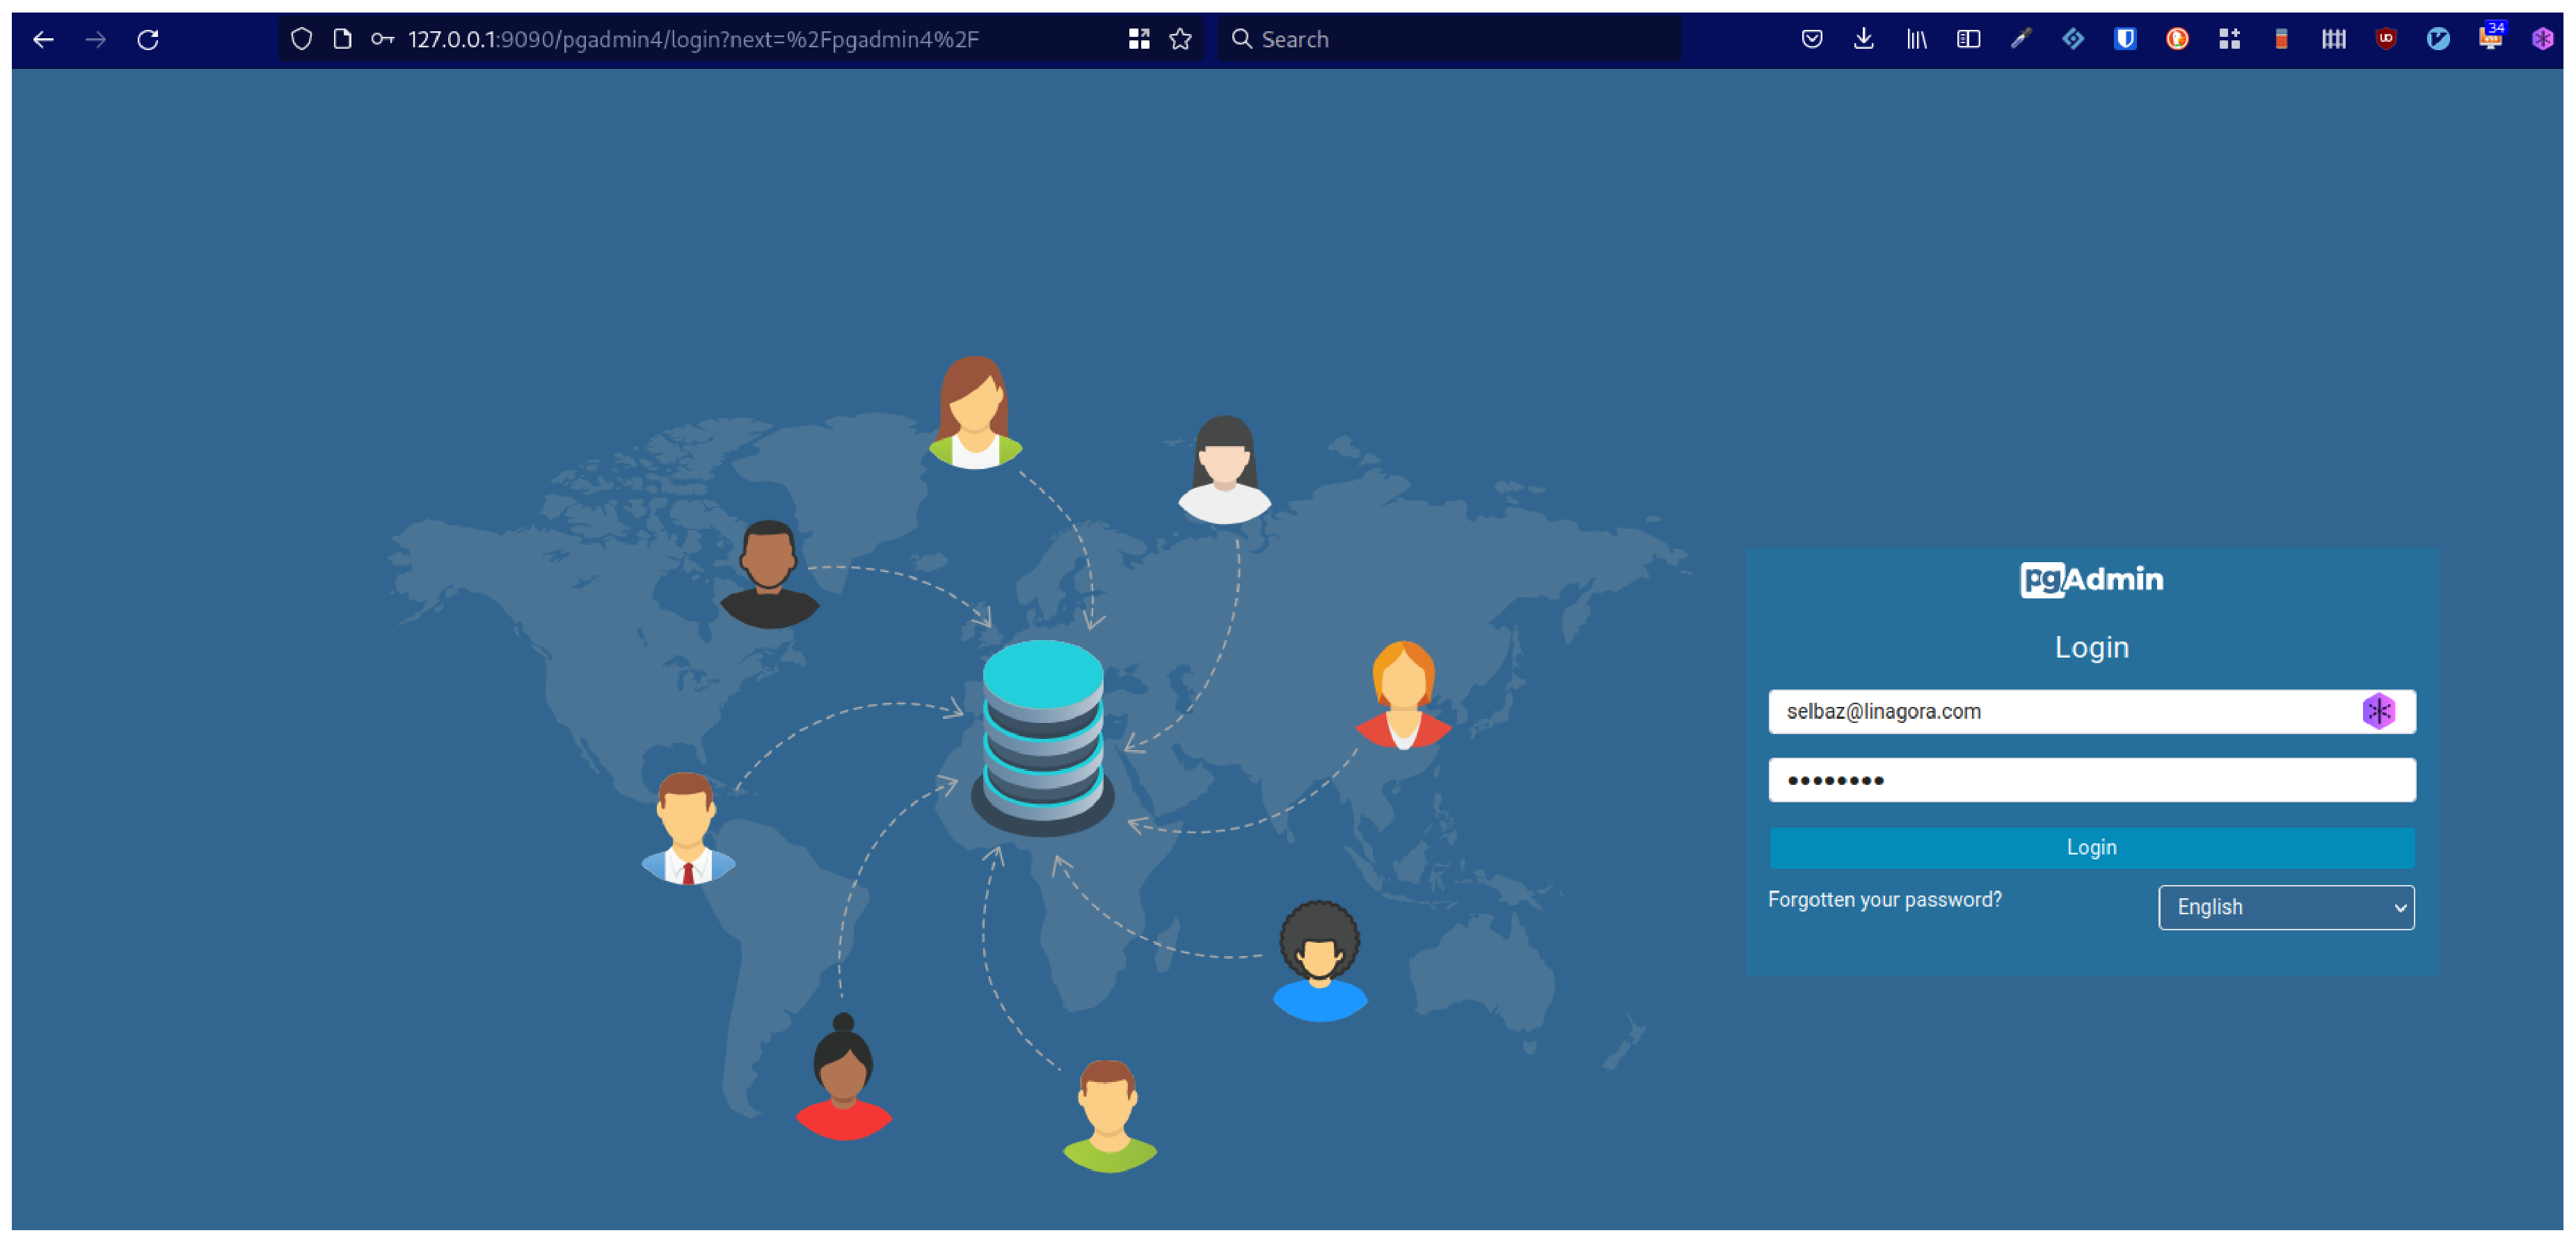
\includegraphics[angle=0, width=0.5\textwidth]{images/pgadmin4_login.eps}
\end{center}
\end{figure}

\begin{figure}
\begin{center}
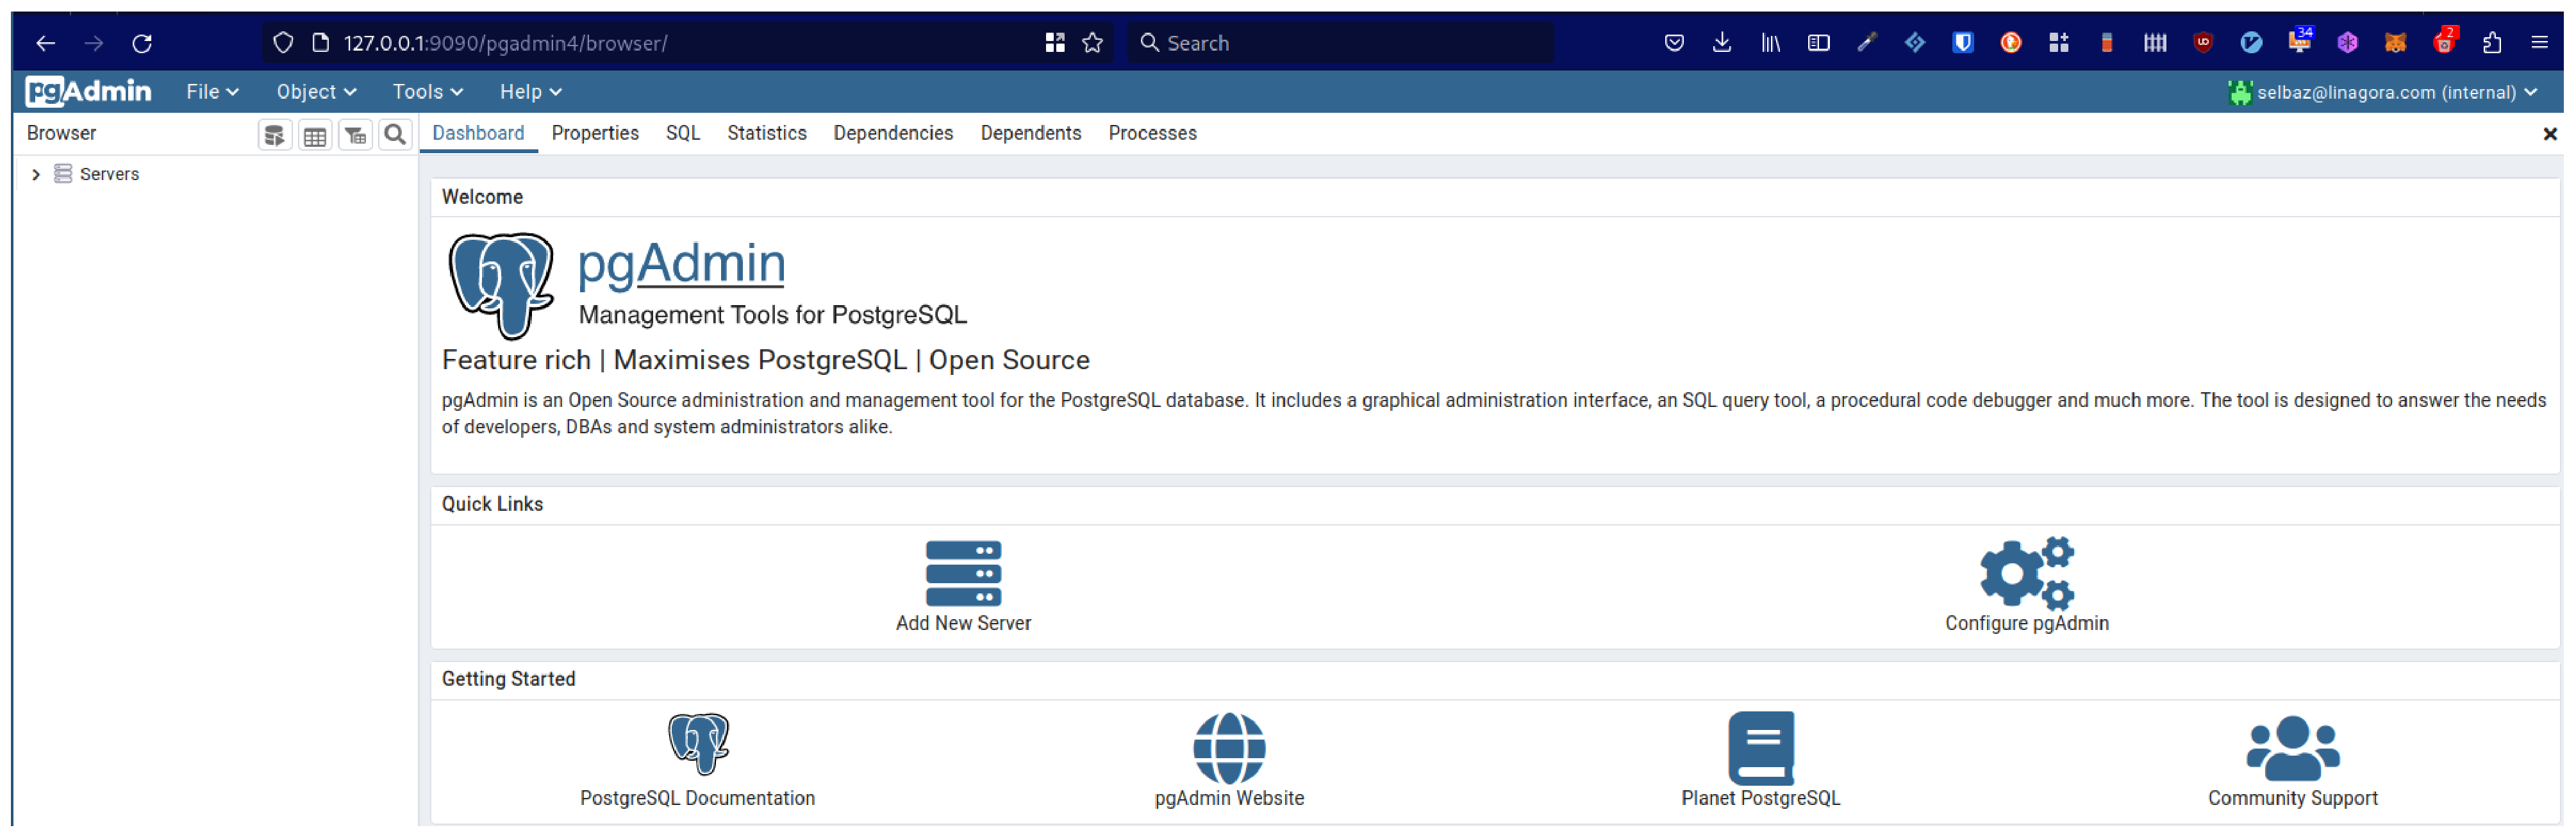
\includegraphics[angle=0, width=0.5\textwidth]{images/pgadmin4_home.eps}
\end{center}
\end{figure}

\end{frame}

%%%%%%%%%%%%%%%%%%%%%%%%%%%%%%%%%%%%%%%%%%%%%%%%%%%%%%%%%%%%%%%%%%%%%%%%%%%%%%%%

\begin{frame}[fragile]{Exercice - pgadmin4 screenshots}

\begin{figure}
\begin{center}
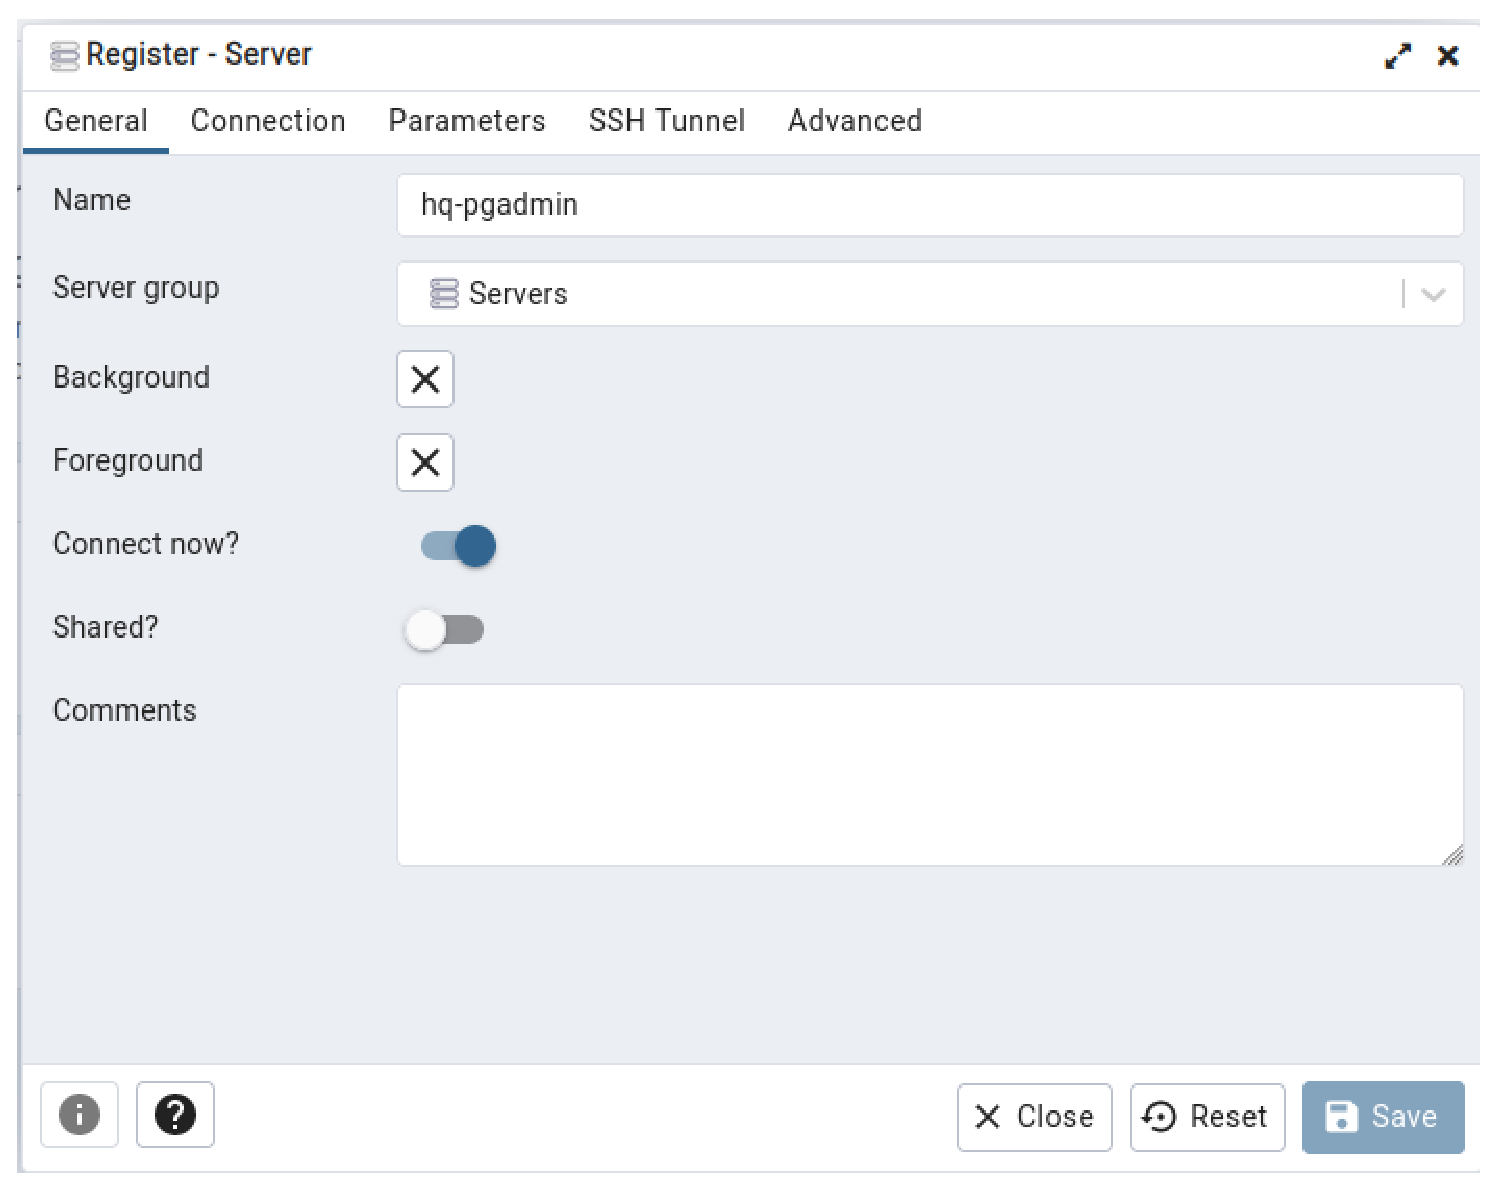
\includegraphics[angle=0, width=0.5\textwidth]{images/pgadmin4_connexiondb.eps}
\end{center}
\end{figure}

\end{frame}

%%%%%%%%%%%%%%%%%%%%%%%%%%%%%%%%%%%%%%%%%%%%%%%%%%%%%%%%%%%%%%%%%%%%%%%%%%%%%%%%

\begin{frame}[fragile]{Le modèle \textbf{template0}}

\begin{itemize}
   \item Le modèle template0 est identique au modèle template1
   \item A la différence de template1, il ne doit jamais être modifié car il représente la base de données à l'état initial
   \item Ce modèle sert de base pour la création de base de données à partir d'un dump généré par \textbf{pg\_dump}
   \item Une autre raison de partir du modèle template0 pour créer une nouvelle base de données, est le changement de jeu de caractères
   \item template0 ne contient pas de choix de jeu de caractères par défaut. Ce qui n'est pas le cas de template1.
\end{itemize}

\end{frame}

%%%%%%%%%%%%%%%%%%%%%%%%%%%%%%%%%%%%%%%%%%%%%%%%%%%%%%%%%%%%%%%%%%%%%%%%%%%%%%%%

\begin{frame}[fragile]{Création d'une base de données à partir d'un modèle}

   Pour créer une base de données à partir du modèle template0, les 2 commandes suivantes sont utilisables au choix:
\begin{tiny}
\begin{Verbatim}[commandchars=\\\{\}]
CREATE DATABASE dbname TEMPLATE template0;
\end{Verbatim}
\end{tiny}
ou depuis le shell:
\begin{tiny}
\begin{Verbatim}[commandchars=\\\{\}]
createdb -T template0 dbname
\end{Verbatim}
\end{tiny}


\end{frame}

%%%%%%%%%%%%%%%%%%%%%%%%%%%%%%%%%%%%%%%%%%%%%%%%%%%%%%%%%%%%%%%%%%%%%%%%%%%%%%%%

\begin{frame}{Généralisation des modèles}

\begin{itemize}
   \item La commande \textbf{CREATE DATABASE} permet de crér une nouvelle base de données en utilisant une autre comme un modèle
   \item Cependant, cet usage est fortement déconseillé
   \item En effet, pendant la copie de la base source, aucune session ne peut se connecter sur la base source
\end{itemize}

\end{frame}

%%%%%%%%%%%%%%%%%%%%%%%%%%%%%%%%%%%%%%%%%%%%%%%%%%%%%%%%%%%%%%%%%%%%%%%%%%%%%%%%

\begin{frame}{La table \textbf{pg\_database}}

\begin{itemize}
   \item La table pg\_database inclut 2 colonnes intéressantes:
   \begin{itemize}
      \item \textbf{datistemplate}: la base peut servir de modèle. Sinon seuls les super-utilisateurs et le propriétaire de la base peuvent s'en servir comme modèle
      \item \textbf{datallowconn}: aucune nouvelle session ne peut être créée.
   \end{itemize}
\end{itemize}

\end{frame}

%%%%%%%%%%%%%%%%%%%%%%%%%%%%%%%%%%%%%%%%%%%%%%%%%%%%%%%%%%%%%%%%%%%%%%%%%%%%%%%%

\begin{frame}{La base de données \textbf{postgres}}

\begin{itemize}
   \item Cette base est une simple copie de template1
   \item Elle sert de base de connexion par défaut pour les utilisateurs et les applications
   \item Elle peut être détruite et recopiée depuis template1
\end{itemize}

\end{frame}

%%%%%%%%%%%%%%%%%%%%%%%%%%%%%%%%%%%%%%%%%%%%%%%%%%%%%%%%%%%%%%%%%%%%%%%%%%%%%%%%

%\section{Jeu de caractères}
%
%%%%%%%%%%%%%%%%%%%%%%%%%%%%%%%%%%%%%%%%%%%%%%%%%%%%%%%%%%%%%%%%%%%%%%%%%%%%%%%%%
%
%\begin{frame}[fragile]{Ensemble de jeu de caractères}
%
%\begin{itemize}
%   \item WIP
%\end{itemize}
%
%\begin{toile}
%\toileurl{https://www.postgresql.org/docs/15/charset.html}
%\end{toile}
%
%\end{frame}
%
%%%%%%%%%%%%%%%%%%%%%%%%%%%%%%%%%%%%%%%%%%%%%%%%%%%%%%%%%%%%%%%%%%%%%%%%%%%%%%%%%
%
%\begin{frame}[fragile]{Changement du jeu de caractères}
%
%\begin{itemize}
%   \item WIP
%\end{itemize}
%
%\end{frame}
%
%%%%%%%%%%%%%%%%%%%%%%%%%%%%%%%%%%%%%%%%%%%%%%%%%%%%%%%%%%%%%%%%%%%%%%%%%%%%%%%%%

\newlength{\largeurtableau}
\setlength{\largeurtableau}{\textwidth}
\addtolength{\largeurtableau}{-2\leftmarginii}

%%%%%%%%%%%%%%%%%%%%%%%%%%%%%%%%%%%%%%%%%%%%%%%%%%%%%%%%%%%%%%%%%%%%%%%%%%%%%%%%
